\documentclass[10pt,a4paper]{article}
\usepackage[utf8]{inputenc}
\usepackage[italian]{babel}
\usepackage{amsmath}
\usepackage{amsfonts}
\usepackage{amssymb}
\usepackage[left=1cm,right=1cm,top=1cm,bottom=1cm]{geometry}

\usepackage{blindtext}
\usepackage[T1]{fontenc}
\usepackage[utf8]{inputenc}

\usepackage{titlesec}
\setcounter{secnumdepth}{4}
\titleformat{\paragraph}
{\normalfont\normalsize\bfseries}{\theparagraph}{1em}{}
\titlespacing*{\paragraph}
{0pt}{3.25ex plus 1ex minus .2ex}{1.5ex plus .2ex}

\usepackage{graphicx}
\usepackage{subcaption}

\usepackage{wrapfig}


\begin{document}

\subsection{Il kinect}

Il kinect \`e \ un dispositivo per la rilevazione del movimento prodotto da Microsoft e commercializzato con la console di gioco Xbox, pu\`o per\`o essere modificato per poterlo interfacciare ad un comune pc.

\begin{wrapfigure}{r}{0.5\textwidth}
  \begin{center}
    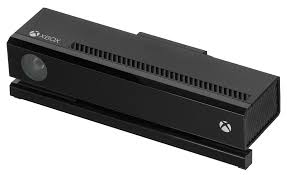
\includegraphics[width=0.5\textwidth]{kinect.jpg}
  \end{center}
  \caption{Il kinect}
\end{wrapfigure}

\end{document}